\documentclass[../AnalysisNoteJBuxton.tex]{subfiles}
\begin{document}

\subsection{Pair Selection}
\label{PairSelection}

It is important to obtain true particle pairs in the analysis.  In particular, contamination from pairs constructed with split or merged tracks, and pairs sharing daughters, can introduce an artificial signal into the correlation function, obscuring the actual physics.  We impose the following pair cuts to combat these issues:

\begin{enumerate}
 \item Shared Daughter Cut for Pairs
 \begin{enumerate}
  \item V0-V0 Pairs (i.e. \LamKs analyses)
  \begin{itemize}
   \item Remove all pairs which share a daughter 
   \begin{itemize}
    \item Ex. \Lam and \Ks particles which share a $\pi^{-}$ daughter are not included
   \end{itemize} 
  \end{itemize}
  \item V0-Track Pairs (i.e. \LamKpm analyses)
  \begin{itemize}
   \item Remove pairs if Track is also used as a daughter of the V0
   \begin{itemize}
    \item In these analyses, this could only occur if, for instance, a K is misidentified as a $\pi$ or p in the V0 reconstruction
   \end{itemize}
  \end{itemize}
  \item $\Xi$-Track Pairs
  \begin{itemize}
   \item Remove pairs if Track is also used as a daughter of the $\Xi$
   \begin{itemize}
    \item In these analyses, this could only occur if, for instance, a K is misidentified as a $\pi$ or p in the V0 reconstruction, or misidentified as bachelor $\pi$.
   \end{itemize}
  \end{itemize}  
 \end{enumerate}
 \item Average Separation Cuts (AvgSep)
 \begin{itemize}
  \item Used to cut out splitting and merging effects
  \item The motivation for these cuts can be seen in Figures \ref{fig:AvgSepLamK0}, \ref{fig:AvgSepLamKch}, and \ref{fig:AvgSepXiKch}, in which average separation correlation functions are presented
 \end{itemize}
 \begin{enumerate}
  \item \LamKs Analyses
  \begin{itemize}
   \item AvgSep $>$ 6.0 cm for like charge sign daughters
   \begin{itemize}
    \item ex. p daughter of \Lam and $\pi^{+}$ daughter of \Ks
   \end{itemize}
   \item No cut for unlike-sign daughters
  \end{itemize}
  \item \LamKpm Analyses
  \begin{itemize}
   \item AvgSep $>$ 8.0 cm for daughter of \LamALam sharing charge sign of \Kpm
   \begin{itemize}
    \item ex. in \LamKchP analysis, p daughter of \Lam with \KchP
   \end{itemize}
   \item No cut for unlike signs
  \end{itemize}
  \item \XiKpm Analyses
  \begin{itemize}
   \item AvgSep $>$ 8.0 cm for any daughter of $\Xi$ sharing charge sign of \Kpm
   \begin{itemize}
    \item ex. in $\Xi^{-}$\KchM analysis, $\pi^{-}$ daughter of \Lam daughter with \KchM, and bachelor $\pi^{-}$ daughter with \KchM
   \end{itemize}
   \item No cut for unlike signs
  \end{itemize}  
 \end{enumerate}
\end{enumerate}

\begin{figure}[h]
  \centering
  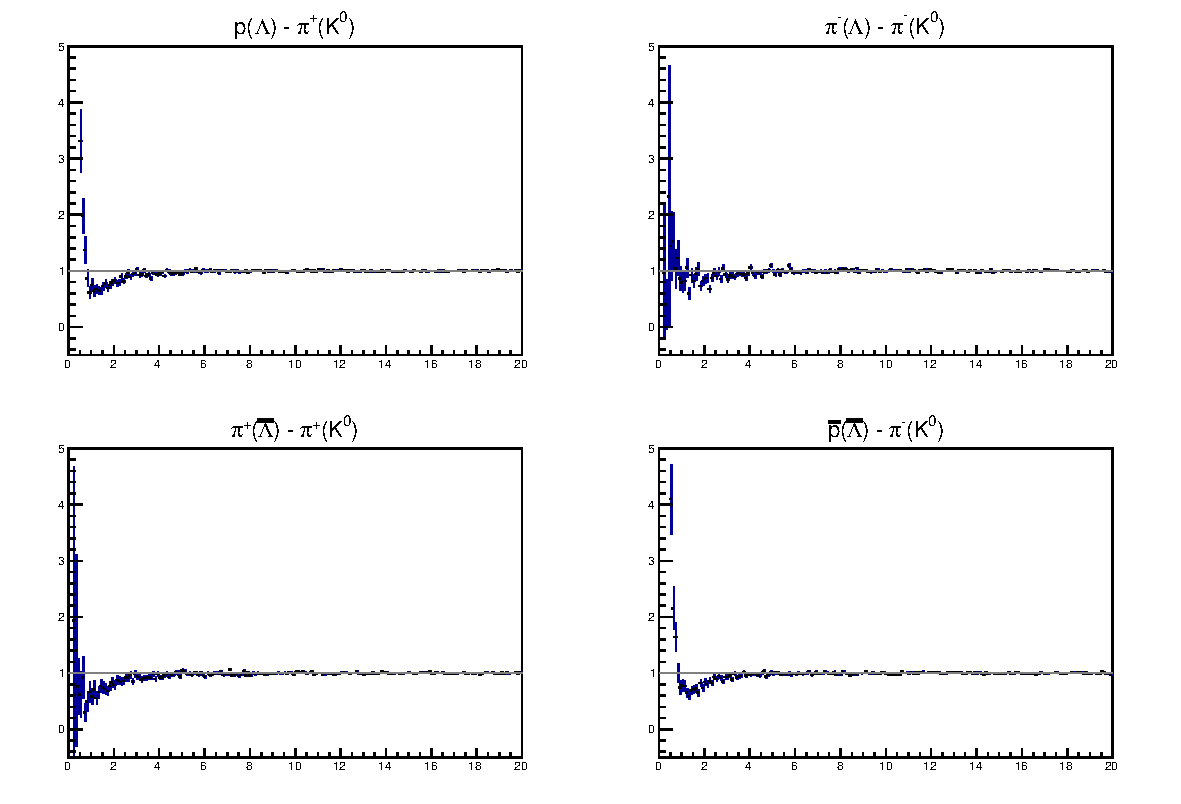
\includegraphics[width=0.8\textwidth]{3_DataSelection/Figures/AvgSepCFs_LamK0.pdf}
  \caption[Avgerage Separation of \LamALam and \Ks Daughters]{Average separation (cm) correlation functions of \LamALam and \Ks Daughters.  Only like-sign daughter pairs are shown (the distributions for unlike-signs were found to be flat).  The title of each subfigure shows the daughter pair, as well as the mother of each daughter (in ``()"),  ex. top left is p from \Lam with $\pi^{+}$ from \Ks.}
  \label{fig:AvgSepLamK0}
\end{figure}

\begin{figure}[h]
  \centering
  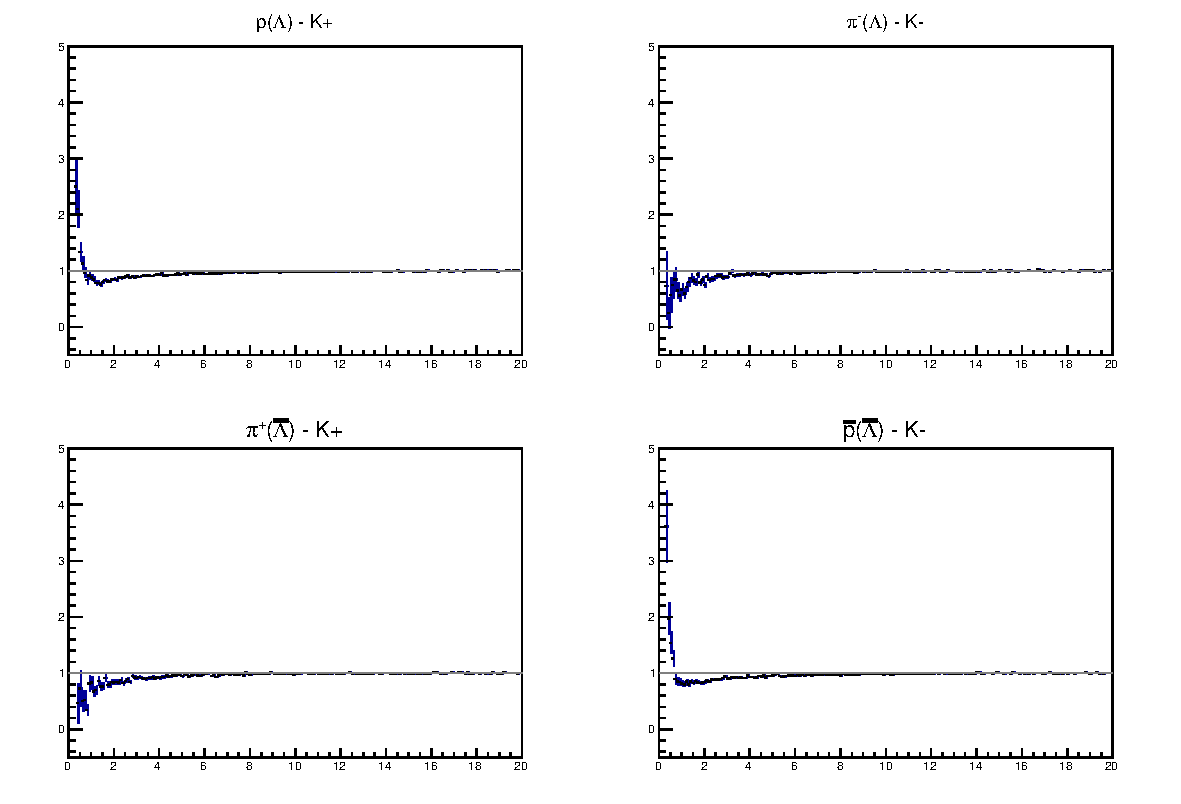
\includegraphics[width=0.8\textwidth]{3_DataSelection/Figures/AvgSepCFs_LamKch.pdf}
  \caption[Avgerage Separation of \LamALam Daughter and \Kpm]{Avgerage separation (cm) correlation functions of \LamALam Daughter and \Kpm.  Only like-sign pairs are shown (unlike-signs were flat).  In the subfigure titles, the particles in ``()" represent the mothers, ex. top left is p from \Lam with \KchP.}
  \label{fig:AvgSepLamKch}
\end{figure}



\begin{figure}[h]
  \centering
  %%----start of first subfigure---  
  \subfloat[$\Xi^{-}$\KchP]{
    \label{fig:AvgSepXiKch:a}
    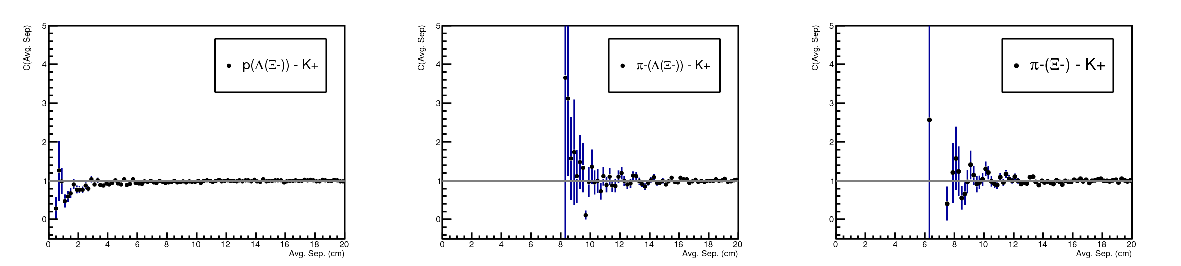
\includegraphics[width=0.99\textwidth]{3_DataSelection/Figures/cXicKchAvgSepCfs_XiKchP.pdf}}\\
  %%----start of second subfigure---
  \subfloat[$\bar{\Xi}^{+}$\KchM]{
    \label{fig:AvgSepXiKch:b}
    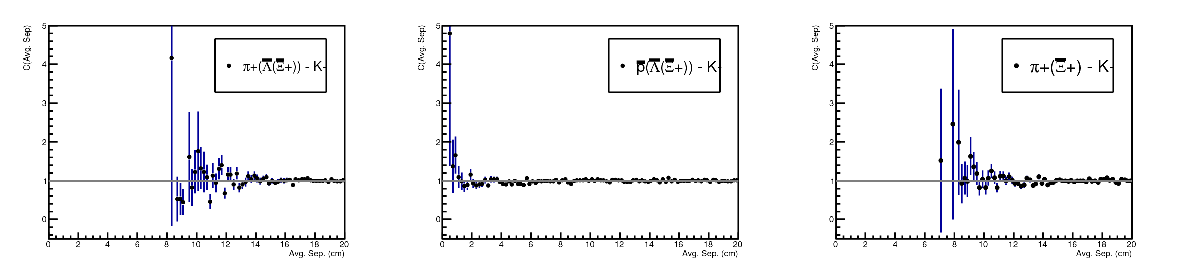
\includegraphics[width=0.99\textwidth]{3_DataSelection/Figures/cXicKchAvgSepCfs_AXiKchM.pdf}}\\
      %%----start of third subfigure---  
  \subfloat[$\Xi^{-}$\KchM]{
    \label{fig:AvgSepXiKch:c}
    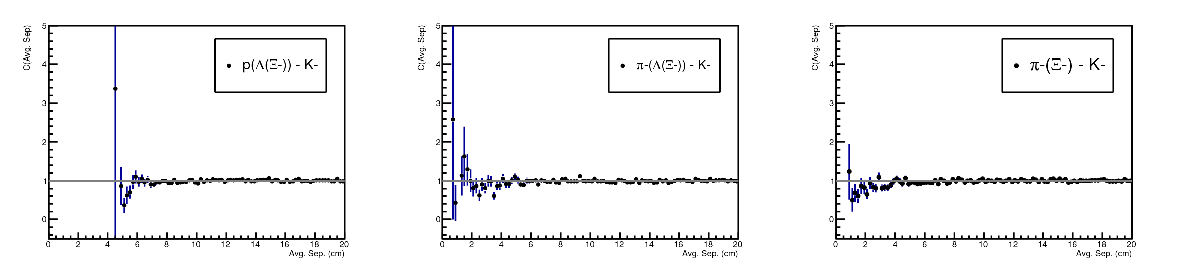
\includegraphics[width=0.99\textwidth]{3_DataSelection/Figures/cXicKchAvgSepCfs_XiKchM.pdf}}\\
  %%----start of fourth subfigure---
  \subfloat[$\bar{\Xi}^{+}$\KchP]{
    \label{fig:AvgSepXiKch:d}
    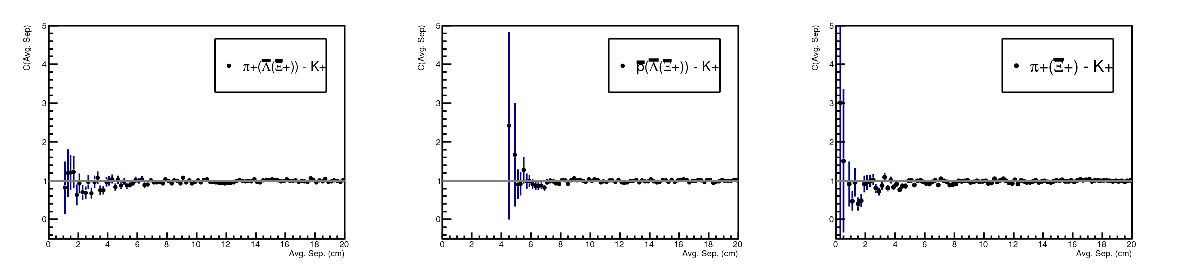
\includegraphics[width=0.99\textwidth]{3_DataSelection/Figures/cXicKchAvgSepCfs_AXiKchP.pdf}}
  %%----overall caption----
  \caption[Avgerage Separation of $\Xi$ Daughters and \Kpm]{Avgerage separation (cm) correlation functions of $\Xi$ Daughter and \Kpm.  In the subfigure titles, the particles in ``()" represent the mothers, ex. top left is p from \Lam from $\Xi^{-}$ with \KchP.}
  \label{fig:AvgSepXiKch}
\end{figure}

\clearpage

\end{document}